\chapter{Basics of Acoustics - Processing Speech}\label{ch-bas-acou}
This section aims to introduce the reader to real-world signals and their representation in Digital Signal Processing (DSP). Such topics as sampling, filtering  and signal analysis fall under the umbrella of DSP. All of the concepts addressed for general signals extend to those of acoustic signals.\\ \\
Acoustic signals are, as in their physical nature, audible signals in continuous time ($t \in \mathbb{R}$). This means that such a signal will vary infinitely over a given length of time. Modelling such complexity in a digital environment, like computing, is infeasible. For this reason the following thesis will restrict it's analysis of signals to the discrete-time domain.

% ======================================================
\section{Sampling - A means of temporal truncation}
\subsection{Sampled Signals}
Sampling refers to taking a continuous-time signal, which is essentially a string of infinite data points in time, an converting the signal to a finite set of numbers. The finite set of data points gathered during the sampling process are collected from the continuous time signal at a finite time interval. This time interval is called the sampling period or sampling interval, $T_0$. If the sampling period is small enough then the sampled signal sufficiently represents the continuous-time signal.\\ \\
Now we must mathematically define the act of sampling. Consider the continuous-time function $x(t)$ such that $t \in \mathbb{R}$. As we wish to sample this signal at a finite sampling interval, we obtain definition \ref{samp_def};
\begin{equation}\label{samp_def}
    x[n] = x(nT_0), \hspace{3mm} n \in \mathbb{N}
\end{equation}
Here $nT_0$ refers to the incremental sampling points with a fixed sampling interval $T_0$. The resulting signal may also be referred to as a discrete-time signal. To construct an alternate definition we may first define the Impulse/Delta function, defined in \ref{delta_def}.
\begin{equation}\label{delta_def}
    \delta(t) =
\left\{
	\begin{array}{ll}
		+\infty  & t=0 \\
		0 & t \neq 0
	\end{array}
\right.
\end{equation}
Whose definite integral is constrained by \ref{delta_cons}. This function will also be referred to as a '\textit{pulse}' throughout this text.
\begin{equation}\label{delta_cons}
    \int_{-\infty}^{\infty} \delta(t) \,dt = 1 \\
\end{equation}
Thus, by multiplying the continuous-time signal $x(t)$ by a shifted series of pulses we obtain the following alternate definition for a sampled function.
\begin{align}\label{samp_def_2}
    x_p(t)  &= x(t) \Big[ \sum_{-\infty}^{\infty} \delta(t - nT_0) \Big] \nonumber \\
            &= \sum_{-\infty}^{\infty} x(nT_0)\delta(t-nT_0)
\end{align}

% ======================================================
\subsection{The Fourier Transform}
The Fourier transform, in a very simplified sense, is a means of taking a signal defined in the time domain and representing it in the frequency domain. For $\omega = 2\pi f$ the Fourier Transform of a continuous-time signal $x(t)$ is defined as in \ref{FT_def}.
\begin{equation}\label{FT_def}
    X(\omega) = \int_{-\infty}^{\infty} x(t) e^{-j\omega t} \, dt
\end{equation}
The inverse of this transform, as one would hope, acts as an inverse mapping between domains. In this case a function in the frequency domain will be mapped back to the temporal domain. See definition \ref{IFT_def}.
\begin{equation}\label{IFT_def}
    x(t) = \dfrac{1}{2\pi} \int_{-\infty}^{\infty} X(\omega) e^{j\omega t} \, d\omega
\end{equation}
The Discrete Time Fourier Transform (DTFT) is one more applicable to digital computing, see \ref{DTFT_def}.
\begin{equation}\label{DTFT_def}
    X(\theta) = \sum_{n = -\infty}^{n = \infty} x[n] e^{-j\theta n}, \hspace{3mm} \theta \in \mathbb{R}
\end{equation}
Nyquist then provides a seminal result for the field of signal processing highlighted in \ref{Nyq1}. He noted that; The discrete-time Fourier transform of a sampled signal is a summation of infinite replicas of the Fourier transform of the original continuous-time signal where each replica is shifted horizontally by an integer multiple of $w_0 = 2\pi / T_0$ \cite{SP_03_textbook}.
\begin{equation}\label{Nyq1}
    X(\theta) = \dfrac{1}{T_0}\sum_{n = -\infty}^{n = \infty} X\Bigg( \dfrac{\theta - 2 \pi n}{t_0} \Bigg), \hspace{3mm} \infty < \theta < \infty
\end{equation}
Thus, the discrete-time Fourier transform can be computed practically after one has computed $X(\omega)$. It is important to note that a result of \ref{Nyq1} is that periodicity will be produced in the frequency domain, caused by the act of sampling.

% ======================================================
\subsection{Nyquist-Shannon Sampling}
We now consider a band-limited function with bandwidth $\omega_b = 2 \pi f_b$ defined by \ref{bl_def}. This is a function such that it only has nonzero values within a specific frequency 'band'. Outside of this band, the frequency domain representation of the function is entirely zero.
\begin{equation}\label{bl_def}
    X(\omega) = 0, \hspace{3mm} |\omega| \geq \omega_b
\end{equation}
For a signal whose bandwidth is $\omega_b$, the \textbf{Nyquist rate} is given by $2f_b$. This is the minimum threshold of which one must sample at to ensure a band-limited signal can be reconstructed from it's samples, as noted by Shannon \cite{SP_03_textbook}. This minimum sampling frequency constraint comes about from the result of \ref{Nyq1}, as mentioned previously. Sampling will produce periodicity in the frequency domain. Thus, one must ensure that the periodic replicas of the original spectrum do not overlap in the frequency domain. Failure to do so will mean that, upon using a Low Pass Filter (LPF) to recover the original spectrum, the spectrum will no longer resemble that of the original band-limited signal $x(t)$. For this reason we always choose a sampling frequency greater than or equal to the Nyquist rate (\ref{Nyq-Shan}). To illustrate this phenomena, refer to figure \ref{Aliases_underSamp}. 
\begin{equation}\label{Nyq-Shan}
    f_0 = \dfrac{1}{T_0} \geq 2f_b
\end{equation}
\begin{figure}
        \centering
        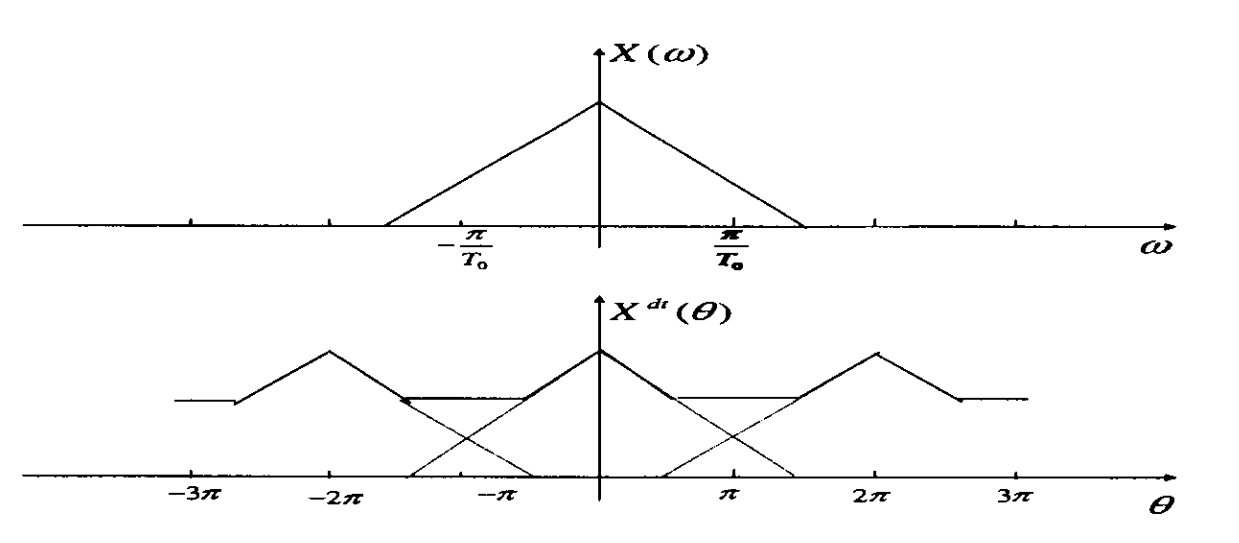
\includegraphics[scale = 1.0]{images/Aliases-under sampled.png}
        \caption{Original spectrum (top) and DTFT and overlapping replicas (bottom) \cite{SP_03_textbook}}
        \label{Aliases_underSamp}
\end{figure}
A corollary of \ref{Nyq-Shan} is that any signal with infinite bandwidth will always have overlapping spectrum replicas. Meaning, reconstruction of such a signal from it's samples is not possible.

% ======================================================
\section{Discrete Time System Classification}
In the simplest terms, a discrete-time system is a transformation, $\mathcal{T}\{\}$, which maps any given input sequence $x[n]$ to an output sequence $y[n]$. This output sequence may be referred to as the system response and is given below.
$$ y[n] = \mathcal{T}\{ x[1], x[2], ..., x[n], ... \} $$

\subsection{Linear Systems}
A linear system is any system under which both \textbf{superposition} properties are always true. These two properties are that of \textbf{scaling} and \textbf{additivity}. The scaling property states that, given an input $x[n]$ that produces an output $y[n]$ under transformation, the same input scaled by a constant will produce the same corresponding output scaled by the same constant. \vspace{-3mm}
\begin{align*}
&\mathcal{T}\{x[n]\} = y[n] \\
&\Longrightarrow \mathcal{T}\{ \lambda x[n]\} = \lambda y[n]
\end{align*}
The additivity property states that the addition of input sequences under transformation will result in the addition of the two corresponding output sequences.
$$\mathcal{T}\{x_1[n] + x_2[n]\} = y_1[n] + y_2[n]$$

\subsection{Time-invariant Systems}
A time-invariant system is one which, under the presence of translation at the input, will produce the same translation at the output.
\begin{align*}
&\mathcal{T}\{x[n]\} = y[n] \\
&\Longrightarrow \mathcal{T}\{ x[n-n_0]\} = y[n-n_0]
\end{align*}

\subsection{Causal Systems}
A causal system is any system for which any given output is not influenced by inputs from the future. An example of a non-causal system would be one such as $y[n_0] = x[n_0 + 1]$, for instance.

\subsection{Stable Systems}
A stable system is one which demonstrates, for a bounded input, a bounded output. This mathematical bound is analogous to limiting the amplitude of a signal, which is commonplace in any quantization process.
\begin{align*}
& |x[n]| \leq B_1 \leq \infty \\
&\Longrightarrow |y[n]| \leq B_2 \leq \infty
\end{align*}

% \subsection{The Linear, Time-Invariant Property}
% ON PAGE 42, INCLUDE IF NECESSARY OR CONVOLUTION IS BROUGHT UP LATER IN THE PAPER.

% ======================================================
\section{Discrete Fourier Transforms}
\subsection{Defining the DFT}
The Discrete Fourier Transform (DFT) is a computationally feasible version of the DTFT. It is obtained by sampling the DTFT in the frequency domain. For a signal with finite sequence length $N$, the DFT is given by definition \ref{DFT_def}.
\begin{align}\label{DFT_def}
    X^d[k]  &= \sum_{n=0}^{N-1}x[n]\exp{\Big( -\dfrac{j2\pi kn}{N} \Big)}, \hspace{3mm} 0\leq k \leq N-1
\end{align}
The key advantage of the DFT is that, by sampling the DTFT at $N$ points, we are able to reconstruct the original signal. The DTFT, on the other hand, required knowledge of the transform at infinitely many points. This is infeasible for a computing system and for this reason the DFT becomes very important. Similarly to the previously defined inverse Fourier transform, the inverse DFT is given in \ref{IDFT_def}.
\begin{align}\label{IDFT_def}
    x[n]  &= \dfrac{1}{N} \sum_{n=0}^{N-1}X^d[k]\exp{\Big( \dfrac{j2\pi kn}{N} \Big)}, \hspace{3mm} 0\leq n \leq N-1
\end{align}
\subsection{Disadvantages of the DFT}
It must be noted, whilst using the DFT, that there is an inherent limit in frequency resolution as opposed to previously mentioned methods. This is because, by analysing a signal of fixed duration $N$, we introduce gaps in between analysed frequencies of width $\Delta \theta = 2 \pi / N$. As is seen from this fraction, the gaps will decrease as the length of the signal increases, also increasing the frequency resolution. However, this poses a large issue for the analysis of short sequences as the resolution in the frequency domain will become severely limited. One such technique to work around this limitation is by using \textbf{zero-padding} to plaster the gaps of the DFT analysis. This will not be discussed in this paper. 

% ======================================================
\section{Short-Time Fourier Transforms}
\subsection{What Necessitates the STFT?}
Typical signal processing methods are performed on signals which are not time varying, and as a result do not change frequency over time. Speech signals, however, are much more complicated than this. As one would be familiar with, when vocalising a complex speech pattern the pitch of your voice may increase and decrease over time. Such is demonstrated in a natural speech signal, which can be characterised by shifting of the signals frequency peaks with respect to time. \\ \\
In such a scenario, an engineer may not want to apply a global transform to an input signal. Such a transform would be representative of those which this paper has concerned itself with up until this point. Instead, one may consider using a number of transforms over smaller intervals of the signal. It is this extension upon previous methods that forms the basis for the Short-Time Fourier Transform (STFT).

\subsection{Defining the STFT}
We may define a windowing function by $w(n-m)$. Such a function is usually symmetric about its midpoint $m=n$. This window function starts near or at zero, then increases to a maximum at the center of the time series and decreases again \cite{heinzel2002spectrum}. Common window functions include Hamming, Hanning and Rectangular windows. After this, the STFT can be defined by \ref{STFT_def}.
\begin{equation}\label{STFT_def}
    X[n, \theta]  = \sum_{m=-\infty}^{\infty} x[m]w[n-m]e^{-j\theta m}, \hspace{3mm} \theta \in \mathbb{R},n \in \mathbb{N}
\end{equation}

\subsection{Multi-Resolution via Spectrogram}
As a STFT is composed of different transforms over a time range, when we take the magnitude of the STFT we do not obtain the same result as for typical Fourier Transforms. Instead we obtain a plot with both a time dimension and a frequency dimension. This is known as a \textbf{spectrogram}. Typically this is plotted by using time as the x-axis, frequency as the y-axis, and colour to indicate the corresponding magnitude at a specific time and frequency. Many contemporary speech recognition and SER machine learning strategies will use some form of spectrogram as inputs, (among other things). They are incredibly useful for deciphering both speech and underlying emotions. One of these graphs, and its corresponding time series counterpart, is depicted in figure \ref{t_spec_plot}.
\begin{figure}
        \centering
        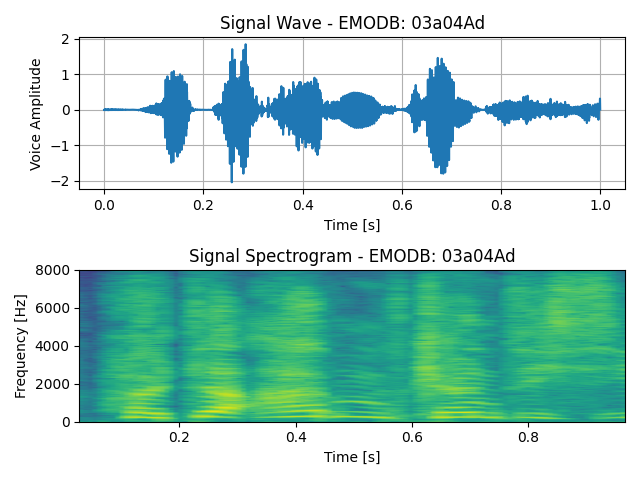
\includegraphics[scale = 0.8]{images/PLOT_TimeANDSpectrogram.png}
        \caption{Spectrogram of emotional speech}
        \label{t_spec_plot}
\end{figure}
It is of important note that the spectrogram does possess its flaws. The window bandwidth (frequency domain) and window time-frame (time domain) are identical under the Fourier transform. It follows that having both a small window bandwidth and small window time-frame, as to capture as much data as is attainable, is not possible. This means that any increase to the granularity of detail in one axis comes at a sacrifice to the detail in the alternate axis. 

% ======================================================
\section{Speech Signals}
Speech can be defined as any acoustic signal, typically created by a human, with frequency content existing within the human range of hearing. This range is approximately from $20Hz$ to $20kHz$. However, realistic ranges are often in between the lower and upper thresholds. As the signal composition of speech is very complicated, speech processing often involves extracting what the engineer deems to be the most useful information. Acoustic signals like speech have many characteristics and deciding which to isolate are application dependent. These extracted characteristics are known as features. As is the case for other domains of machine learning, these features form the basis for analysis and network training. 

\subsection{Speech Signal Analysis - Time \& Frequency Domains}
When analysing speech signals we have the choice to analyse them over a particular domain. That is, we can analyse them over the time domain, frequency domain, or both. Each of these different domains highlight different features and properties of the speech signals. Time and frequency representations of a speech signal taken from the EMODB dataset are illustrated in figure \ref{t_and_f_plot}. \\ \\
When visualising or analysing these signals in the time domain, the signal is referred to as a waveform. The key observable property of the speech in this state is the amplitude as a function of time. This directly relates to the volume or perceived loudness of such a signal. \\ \\
More observable in the frequency domain representation are frequency 'peaks'. These peaks correspond to where the majority of energy is stored in the signal, with respect to frequency. The highest peak would indicate that, across the signal, the most energy is present at or near that particular frequency.
\begin{figure}
        \centering
        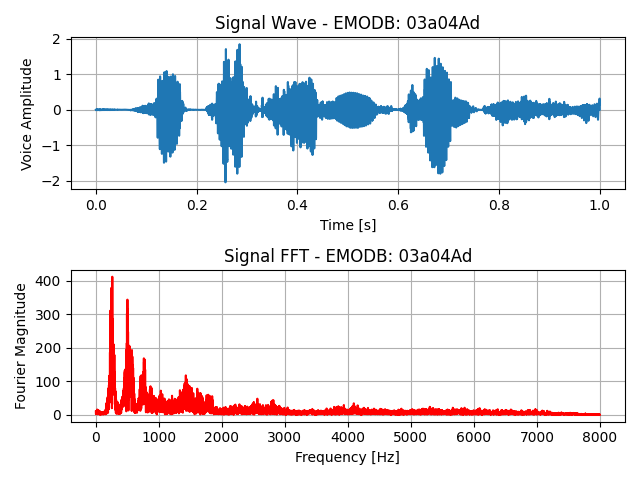
\includegraphics[scale = 0.8]{images/PLOT_timeAndFreq.png}
        \caption{Time and frequency representations of speech}
        \label{t_and_f_plot}
\end{figure}

\subsection{Fundamental Characteristics of Speech}
\begin{description}
\item[Overall Power:]
This is a measure for volume over the duration of the speech signal (or otherwise specified durations). Where amplitude is volume measured at an instant in time, overall power is essentially an average of volume over a range of time. This can give insights to the gender or emotional stress level of a speaker. 

\item[Short-time Power:]
Short-time power, as the name suggests, refers to the power observed over a shorter time frame. It is important to note that due to the linguistic complexity of speech production, speech signals are prone to changing drastically over very small time intervals. To capture this change, it is the role of a processing engineer to divide a signal into small windows of time. In doing so, the rapid and dynamic nature of the acoustic waveform should be roughly captured.\\ \\
Choosing a window length is application dependent due to the inherent trade-off of minimising window length. It would be ideal to have infinitely small time windows, as to capture every microscopic change in dynamic speech. However, this would result in enormous amount of digital processing, which is not computationally feasible. Thankfully, we can use insights from speech pathology to inform us of suitable window lengths which will not overburden a computer. The content of the speech signal can also drastically alter the required size of time windows. For example, long vowels  sounds can be captured with sufficient detail with time-frames of ~100 ms. However, other more abrupt noises may require windows of 5ms to 10 ms \cite{SP_03_textbook}. In general, the vocal tract system of a human deforms at a relatively slow rate. For this reason, the approximation can be made that speech signals do not vary over a window length of $\approx 10ms$ \cite{introtoDSP_core2}. The speech signal over these non-varying windows are referred t as \textit{stationary}.

\item[Fundamental Frequency:]
The fundamental frequency, $F_0$, is conventionally associated with the pitch of the speaker. In terms of SER, it is one of the most revealing features. It is crucial for identifying a subjects intonation; the rise and fall of one's pitch as they produce a speech signal. This intonation can be directly related to a current emotional state.

\item[Frequency Spectrum:]
This refers to the band of frequency of which the signal exists within. For example, if a human male was speaking between frequencies of $200Hz$ and $800Hz$ the spectrum would lie mostly between these two values. This range of frequencies is also known as the bandwidth of a speech signal. An example of the overall frequency spectrum is plotted in the bottom subplot of figure \ref{t_and_f_plot}.

% \item[Short-time average zero-crossing rate:]???

% \item[Short-time autocorrelation function:]???

\end{description}

% ======================================================
% \section{Tracking Speech and It's Formants}
% IN SECTION 2.4 OF TEXTBOOK


% ======================================================
\section{Fundamental Frequency Calculation}
Due to the non-stationary nature of speech (dynamically time-variant), among other factors, the calculation of $F_0$ is rather complex. It is also one of the most formative features of speech signals. Thus, their is a large importance placed upon accurate calculation of the fundamental frequency. 
\\ \\
Speech can, however, be approximated as periodic and stationary over a small enough timescale. As the signal is quasi-periodic, it follows that the fundamental frequency will generate additional harmonics at integer multiples of $F_0$. If one works backwards from the frequency spectrum, by observing the placement of the harmonics one may be able to estimate the fundamental frequency. $F_0$ Can also be calculated through time domain methods, however, this typically yields a lower accuracy \cite{SP_03_textbook}. It does typically provide a means of more efficient computation though. The basic process of estimating pitch is summarised by the subsequent steps.
\begin{itemize}
    \item \textbf{Pre-processing:} This typically involves some kind of filtering or adjustments made to the signal. Such adjustments are made to create a simplified signal which is easier to process.
    
    \item \textbf{Extraction:} This refers to the actual estimation of $F_0$ for the specific signal being analysed at that time. The quantity can be derived from the perspective of the time or frequency domain. 
    
    \item \textbf{Post-processing:} Given that the fundamental frequency obtained is an estimate, this process is prone to errors. This final step involves forms of error correction. This can look like enforcing continuity over the set of calculated frequencies for all windows.
\end{itemize}

% \subsection{Time Domain Calculation}
% \subsection{Frequency Domain Calculation}



% ======================================================
\section{Phonetic Classification of Speech}
While a mathematical classification of speech and its fundamentals is incredibly useful for DSP applications, a phonetic classification is also necessary. Through understanding the physical processes used in the creation of speech, one may better design DSP systems. Notably, this understanding is vital for feature identification.
\\ \\
Speech can be classified as a pressure based waveform, traditionally created by a human. Most people relate speech waveforms to a signal emitted from one's mouth. While this is correct, the signals are created by complicated processes also involving the vocal tract, nostrils, and other body parts. All of these body parts will vibrate in specific ways, creating sound. Among the main tools shaping the speech output are the vocal tract and vocal cords. They are responsible for volume and pitch of the emitted signal. These sounds can be analysed on a 'chunk by chunk' basis. The resulting fragmented speech chunks are referred to as \textbf{phones}. The most fundamental unit of speech is a \textbf{phoneme}. These are essentially distinct sounds, used to differentiate words and larger units of speech from one another. Phones are the acoustic, audible counterparts of phonemes. In order to create a particular phoneme verbally, one must correctly position their jaw, teeth, tongue, velum, lips and their vocal cords. It is simple to see, upon further inspection, how complicated the speech generation process is mechanically, via the necessary collaboration of so many articulatory systems. Phonemes can generally be classed as one of two categories in speech processing. The first category of phonemes is vowels. These typically manifest as more intense sounds. The second category is consonants. These phonemes impose a constriction on the vocal tract and limit the airflow through it. On the contrary, vowels impose no limit on vocal tract airflow.

